\chapter{Integration Notes}

\section{Integration into a Project}
\ifnum \DocumentGroup=1{
Please refer to the installation instructions included in the RTA-SUM Getting Started Guide to generate the RTA-SUM LNM directly inside ISOLAR-AB.
Briefly you can select RTA Code Generator for configuring the SUM Modules that want to be integrated in the project accordigly to its Model Year (MY) version. 
When the option \textit{Not Configured} is selected, the module will not be integrated.
}
\else{
There is no need for standard installation procedure for LNM. The folder itself contains all the necessary
artifacts to integrate into a project. Dropping the complete folder structure into a BSW configuration
project will enable the user to configure LNM and generate all the necessary artifacts.
}\fi

Refer to \href{https://rtahotline.etas.com/confluence/display/RH/RTA-SUM}{RTA-SUM Knowledge Base} for more details about how to integrate this module into a project.

\section{Module Dependencies}

\section{Configuring LNM}
Once the complete package has been added to your project, an additional module RTA-SUM LNM should appear. 
From here you can open and begin configuring the module. 
Specific descriptions of each configurable parameter available are available in the "Description" view of 
\ifnum \DocumentGroup=1
{
ISOLAR-B
}
\else
{
ISOLAR-A with BCT add-on
}\fi when a parameter is selected.

\section{Generating Artifacts}
Generating the C/H/SWCD files from your configuration is similar to other BSW modules delivered from ETAS.
The Code Generation perspective of the 
\ifnum \DocumentGroup=1
{
ISOLAR-B
}
\else
{
ISOLAR-A with BCT add-on
}\fi , should present the user with a dialog to select specific module within the project to generate.
\ifnum \DocumentGroup=1
{
%Nothing
}
\else
{
Either a Partial Build or Full Build can be used, depending on the needs of the user.
}\fi 
In case of any configuration errors present in LNM, the console window will output a description of any errors found during generation.
Further, when the user is configuring the module, the Problems Log will show any active errors in the configuration of LNM.
A third visual aid is the appearance of red X’s in the configuration view over items which are invalid.
Simply hovering over these X’s will provide the user a description of the problem.
These are static validations.

\section{Configuring the RTE}
After the user has configured and generated the artifacts for LNM, the outputted SWCD file \linebreak(\file{SUM\_LNM\_Swcd.arxml}) can be used for the RTE configuration. 
This is a complete SWC description per the AUTOSAR standard of all the users configured ports and interfaces required for the project specific configuration. 
This SWCD is a standard ASW component and not a module description. Therefore, there are no special considerations to be taken into account when configuring the RTE. 
It is recommended that if specific changes are required to the SWCD, the user not manually edit this file, rather update and regenerate the configuration with the required changes.


Note: RTE command used for RTE generation

\begin{rtecommandline}
-err=xml -nts --samples=memmap --os-define-osenv=RTAOS40 
--exclusive-area-optimization=disable --os-output-param=all 
--strict-unconnected-rport-check=off --strict-initial-values-check=warn
\end{rtecommandline}

\chapter{Module Configuration}
This chapter will describe some calibration and configuration parameters and helpful hints for configuring it.

\section{Configuration Parameters}
\subsection{LNM Containers}
\label{sec:LNM Containers}
RTA-SUM LNM parameters are divided in three containers (Figure \ref{fig:containergeneral}): LNMGeneral, LNM\_Networks and LNMArbitration.
\begin{figure}[h!]
\begin{center}
	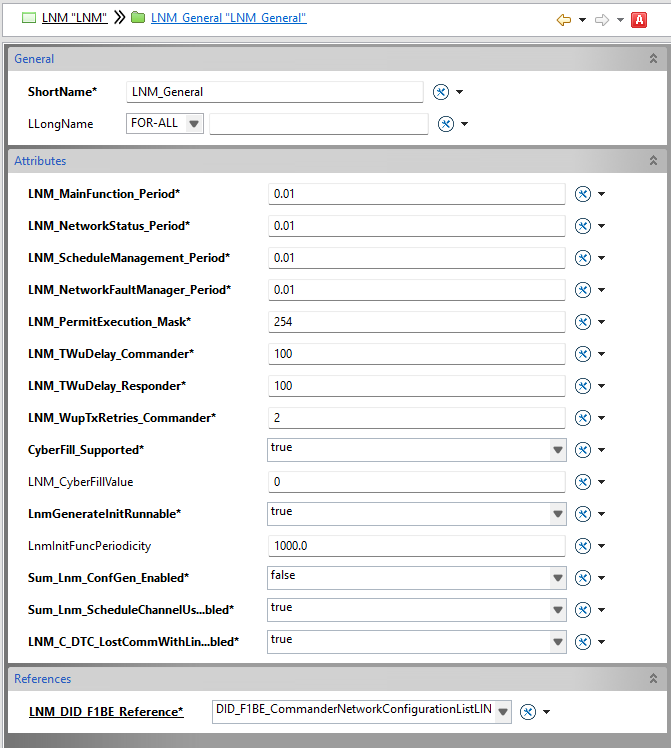
\includegraphics[width=0.9\textwidth]{images/params}
      \caption{RTA-SUM LNM Containers' architecture}
  \label{fig:containergeneral}
\end{center}
\end{figure}

\newpage
\textbf{LNM\_General}\newline
Defines the general parameters for LNM

\quad\quad \textbf{LNM\_MainFunction\_Period}\newline
\null\qquad Time in s, range [0.001;0.2]s, for the periodicity of the MainFunction runnable.

\quad\quad \textbf{LNM\_NetworkFaultManager\_Period}\newline
\null\qquad Time in s, range [0.001;0.2]s, for the periodicity of the NetworkFaultManager.

\quad\quad \textbf{LNM\_NetworkStatus\_Period}\newline
\null\qquad Time in s, range [0.001;0.2]s, for the periodicity of the NetworkStatus. 

\quad\quad \textbf{LnmGenerateInitRunnable}\newline
\null\qquad Defines whether a Runnable shall be generated to call the module's init function.

\quad\quad \textbf{LnmInitFuncPeriodicity}\newline
\null\qquad Defines time in ms for the periodicity of the runnable Runnable\_LNM\_Init

\quad\quad \textbf{LNM\_C\_DTC\_LostCommWithLinResp\_Enabled}\newline
\null\qquad Defines the initial value of the calibration parameter to enable the Lost Communication with \newline
\null\qquad LIN Responder Device DTC aggregation.

\textbf{LNM\_Network}\newline
Defines the configuration of the LNM Networks

\quad\quad \textbf{LNM\_ScheduleManagement}\newline
\null\qquad Defines the configuration of the schedule state machine of the selected LNM Network

\qquad\qquad \textbf{LNM\_ScheduleStates}\newline
\null\qquad\qquad Defines the configuration of the project specific schedule states of the selected LMN Network

\qquad\qquad \textbf{LNM\_ScheduleTransitions}\newline
\null\qquad\qquad Defines the configuration of the possible transition between the different schedule states \newline
\null\qquad\qquad of the selected LMN Network

\textbf{LNM\_Arbitration}\newline
Defines the configuration of all the project specific logic implemented in LNM

\qquad \textbf{LNM\_Inputs}\newline
\null\qquad Defines all the possible inputs to SUM\_LNM that can be used for project specific logic configuration

\qquad \textbf{LNM\_Conditions}\newline
\null\qquad Defines configuration of simple logic operation based on a single LNM\_Input

\qquad \textbf{LNM\_Rules}\newline
\null\qquad Defines configuration of complex logic operation based on LNM\_Conditions and LNM\_Rules


\section{Configuration Hints}

\subsection{Mandatory Parameter Validation}
\label{sec:inputvalidation}
RTA-SUM LNM performs input validation on the ARXML BAMF configuration parameters.
If a mandatory parameter is not configured, RTA-CAR will stop the code generation and report an error identifying the missing or invalid parameter.

Ensure all mandatory parameters are properly set before executing the code generation. The following behavior applies:

\begin{itemize}
	\item If a mandatory parameter is missing or left unconfigured, RTA-CAR halts the generation and outputs an error message specifying the affected parameter.
	\item The generation will not proceed until all mandatory parameters are correctly provided.
	\item Review the reported error to identify and resolve any missing or invalid parameter configuration.
\end{itemize}

\begin{figure}[h!]
	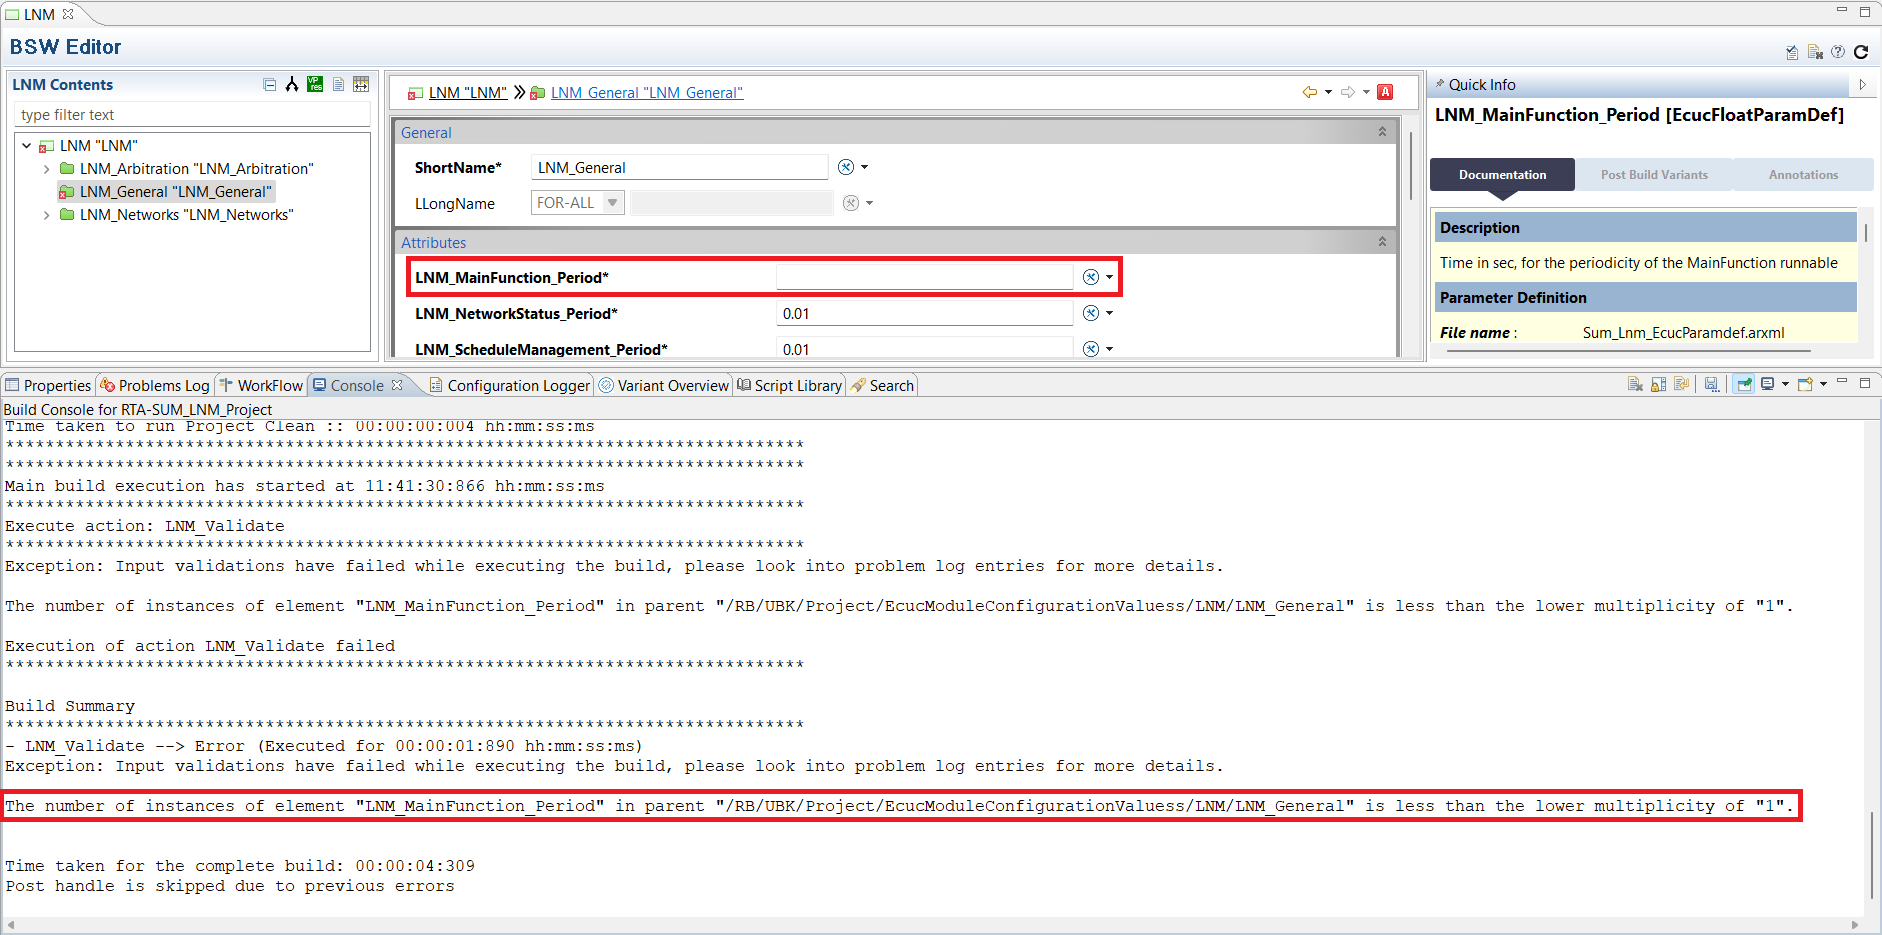
\includegraphics[width=1\textwidth]{images/MandatoryParamMissing.png}
	\caption{RTA-CAR error example for missing mandatory parameter.}
	\label{fig:MandatoryParamMissing}
\end{figure}

\subsection{LNM Initialization}
\label{subsec:init}
To initialize correctly the module, there are two paths that the user can use based on the configuration of the boolean \textbf{LnmGenerateInitRunnable} parameter.


If it is FALSE the user shall invoke the SUM\_LNM initialization function \code{LNM_Init()}, which is an external function declared in the header file \file{SUM_LNM_MainFunction.h}.
The BswM shall invoke this function at initialization time through a BswMAction.


If it is TRUE, the user shall schedule the runnable \code{Runnable_LNM_Init} in a lower periodicity OS task.

\subsection{LNM MainFunction}
\label{subsec:LNM MainFunction}
SUM LNM Main Function is responsible for the management of the PermitExecution, ShutdownPermission and checking VehiclePowerMode, and manages the internal state of SUM LNM. It is also responsible for triggering evaluation of activation rules for the LIN Networks that are activated by rule whose conditions include VehiclePowerMode. Furthermore, SUM LNM is intended to be a supervised entity. The main function is responsible for notifying the aliveness of the module to the WdgM.


It is possible to configure the periodicity of these operations through the configuration parameter \code{LNM_MainFunction_Period}.


The user shall configure SUM SUSD in order to generate the PermitExecution, ShutdownPermission and VehiclePowerMode interface to the SUM LNM. When the SUM modules are generated the user shall connect \code{RP_SUSD_LNM_PermitExecution} to the respective PPort generated by SUM SUSD, \newline \code{PP_LNM_SUSD_ShutdownPermission} to the respective RPort generated by SUM SUSD \newline and \code{RP_SUSD_LNM_VehiclePowerMode} to the respective PPort generated by SUM SUSD.


SUM LNM will transition to the RUNNING state when the PermitExecution relevant bits are set to 1 by SUM SUSD. It is possible to configure which are the relevant bits through the configuration parameter \code{LNM_PermitExecution_Mask}. The user shall put the value of the bit mask into this field, where, the bits set to 0 are relevant for the transition to the RUNNING state, while the bits set to 1 are \code{don't care} for this transition.


Example: \textit{LNM\_PermitExecution\_Mask = 254 (i.e. 0xFE)} means that only the LSB will be used for the transition to the \textit{RUNNING} state. This means that when SUM SUSD sets to 1 the wakeup bit, SUM LNM immediately transitions to the RUNNING state.


SUM LNM is a WdgM supervised entity. This means that a new supervised entity shall be configured in WdgM for SUM LNM. This supervised entity shall have a unique checkpoint. The user shall connect \code{RP_WdgM_LNM_LocalSupervision} to the respective WdgM port.

\subsection{Cyberfill}
SUM LNM provides the Cyberfill value at initialization. This functionality can be turned on or off at configuration time. To support this functionality the user shall set the configuration parameter \code{CyberFill_Supported} to true, and configure the cyberfill value to be provided by setting the parameter \code{LNM_CyberFillValue}. The cyberfill value will be provided through the port \code{PP_LNM_Cyberfill}.

\subsection{Network activation / deactivation}
\label{subsec:Network activation}
SUM LNM manages all the networks that are configured through the container \code{LMN_Networks}. For each of the network configured, SUM LNM manages its activation and deactivation. Activation and deactivation criteria are project specific. Activation criteria can either be a single activation signal (data type uint8) or a rule (set of conditions linked together) for each network.

\begin{itemize}
\item The activation's signal source is configurable through the parameter \code{LNM_ActivationSignalType}
\item Activation criteria of the network as a rule is configurable through the parameter \newline\code{Sum_LNM_Rule_ref}
\item Activation criteria of the network as a single signal is configurable through the parameter \newline\code{LNM_ActivationMask}
\item Deactivation criteria of the network as a single signal is configurable through the parameter \code{LNM_DeactivationMask}
\end{itemize}


To receive correctly the activation signal the port \code{RP_LNM_ActivationSignal_<n>} shall be connected to the respective activation signal port provider. If the activation signal is provided from the Com, the additional port \code{RP_LNM_ActivationSignal_Av_<n>} shall be connected to the respective SUM SSM port that provides the availability indication for that signal.

The logic of the activation and deactivation of the network channel with a rule depends on the evaluation of the defined rule. In particular:
\begin{itemize}
\item The network will be activated if the rule will return true
\item The network will be deactivated if the rule will return false
\end{itemize}
The logic of the activation and deactivation of the network channel with a single activation signal is similar to the PermitExecution (section 2.2). In particular:
\begin{itemize}
\item The network will be activated if all the relevant bits in the activation mask are set to 1
\item The network will be deactivated if all the relevant bits in the deactivation mask are set to 0
\end{itemize}


Please notice that SUM LNM reacts to an activation signal notification as a Data Received Event, i.e., the occurrence of any activation signal notification has the highest priority. An activation or deactivation request must be notified only once to SUM LNM.
SUM LNM requests the activation and deactivation of the LIN Network through the port \code{PP_LNM_BswM_ComM_RequestComMode_<n>}. The user must connect this port to the BswM. BswM shall be configured to react to this mode switch in order to correctly activate and deactivate the LIN channel upon a SUM LNM request.


Mode switch interface:
\begin{itemize}
\item \textit{NOCOMM} request: the BswM shall perform actions to deactivate the LIN channel
\item \textit{FULLCOMM} request: the BswM shall perform actions to activate the LIN channel
\end{itemize}


For the correct functionality, SUM LNM shall be always notified of the current LIN channel state from the BswM through the port \code{RP_LNM_BswM_LinSM_CurrentState<n>}. This means that the BswM shall be configured to receive any channel state update and to update accordingly the mode switch interface used for SUM LNM notification.


Mode switch interface:
\begin{itemize}
\item \textit{NOCOMM} switch: the BswM shall switch the mode to this state when BswM is notified that the LIN channel transitioned to the NO COMMUNICATION state.
\item \textit{FULLCOMM} switch: the BswM shall switch the mode to this state when BswM is notified that the LIN channel transitioned to the FULL COMMUNICATION state.
\end{itemize}

\subsection{Schedule management}
\label{subsec:SchMgnt}
SUM LNM implements a Finite State Machine (FSM) to manage the schedule tables for each configured LIN channel.


Each state of the FSM is associated to a specific schedule table, except to two specific states: the \textit{START} state, which is not associated to any schedule table, and the \textit{SLEEP} state that is associated with the \textit{NULL} schedule. These two states are mandatory and must be configured in any configuration.


To support project specific needs, the user can configure several schedule states for each LIN network by configuring the container \code{LNM_ScheduleState} and providing for each of this states the reference to the respective schedule table \code{LNM_ScheduleRef}.


The logic to transitions between the different states is project specific. SUM LNM supports the possibility to create a link between two states by configuring the \code{LNM_ScheduleTransition} container. For each transition a reference to the starting state must be provided \code{LNM_StartStateRef} as well as a reference to the end state \code{LNM_EndStateRef} and a reference to a logical expression (checked periodically) that must be satisfied to transition from the start state to the end state. (See section 2.6 for details on configuration of the logical expressions).


Please notice that when the \textit{SLEEP} state is entered, the \textit{NULL} schedule is requested, as well the {NO COMMUNICATION} of the LIN channel. At this point, a new commander (or responder) activation of the LIN channel is needed.


SUM LNM requests a schedule table to the BswM module through \newline the port \code{PP_LNM_BswM_LinSM_ScheduleRequest_<n>}. The user must connect this port to the BswM and must configure the BswM in order to react to the mode switch with a schedule request to the LinSm.
When configuring the BswM Action List, the parameter \code{BswMActionListExecution} must be set to \code{BSWM_CONDITION}.

Mode switch interface:
\begin{itemize}
\item \textit{NULL\_SCHEDULE}: BswM shall request the 	\textit{NULL} schedule when entering this state
\item \textit{<ProjectSpecificState>}: BswM shall request the schedule table associated to the specific state
\end{itemize}


For the correct module functionalities, SUM LNM makes use of the current schedule feedback from BswM through the port \code{RP_LNM_BswM_LinSM_CurrentSchedule_<n>}.


Mode switch interface:
\begin{itemize}
\item \textit{NULL\_SCHEDULE}: BswM shall switch to this value when the current stored schedule table is the \textit{NULL} schedule
\item \textit{<ProjectSpecificState>}: BswM shall switch to this value when the current stored schedule table is the one associated to the project specific state
\end{itemize}

\textbf{Pre-Sleep Calibration Parameter and Schedule Management}

To ensure the pre-sleep feature operates as expected, \texttt{LNM\_C\_PreSleepDelay} (in ms) must be the same as or a multiple of \texttt{LNM\_NetworkStatus\_Period} (in sec).

\subsubsection*{Parameters}

\begin{itemize}
    \item \textbf{LNM\_C\_PreSleepDelay}:
    \begin{itemize}
        \item Delay from the criteria satisfaction to transition to NULL schedule.
        \item Maximum: 4000 ms
        \item Default: 25 ms
    \end{itemize}
    \item \textbf{LNM\_NetworkStatus\_Period}:
    \begin{itemize}
        \item Period for checking network status (in seconds).
    \end{itemize}
\end{itemize}

\textbf{Note}: Convert \texttt{LNM\_NetworkStatus\_Period} to milliseconds (e.g., 2 sec = 2000 ms) and ensure \texttt{LNM\_C \_PreSleepDelay} matches or is a multiple of this value for proper pre-sleep functionality.

\subsection{Configuration of project specific logical expressions}
\label{subsec:ProjSpecificLogicExp}

SUM LNM supports the possibility to create project specific logical expression that needs \newline to be checked during the execution of its functionalities (e.g. check project specific conditions to transition from one state to another during the schedule management). Each logical expression is a complex logical composition between different inputs, which create the so-called \code{LNM\_Rule}.


A \code{LNM\_Rule} is a logical aggregation of simpler conditions based on a single input signal, that are the so called \code{LNM\_Condition}.

A \code{LNM\_Condition} compares an input signal to a predefined value. To configure a condition, the following fields must be configured:

\begin{itemize}
\item \textit{LNM\_InputRef} : a reference to the input signal that must be checked
\item \textit{LNM\_CompareValue} : the predefined value to which the input signal is compared for signal types other than VPM
\item \textit{LNM\_CompareVPMValue} : the predefined value to which the input signal is compared for VPM signals
\item \textit{LNM\_CompareOperator} : the operator used to compare the input signal and the predefined value
\end{itemize}


SUM LNM assumption for boolean values condition configuration: FALSE = 0 and TRUE = 1.


Multiple \code{LNM_Condition} connected with a logical operator (AND or OR) creates a \code{LNM_Rule}, as depicted in Figure \ref{fig:rule}. To configure a rule it must be provided a list of conditions \code{LNM_ConditionRef}, and the logical operator to connect them \code{LNM_LogicOperator}.


Exception: it is possible to create rule composed by a single \code{LNM_Condition}. In this case the logical operator \code{LNM_LogicOperator} is not mandatory.


It is possible to reference a \code{LNM_Rule} inside the list \code{LNM_ConditionRef}. This allows to create complex logical expressions.

\begin{figure}[h!]
\begin{center}
	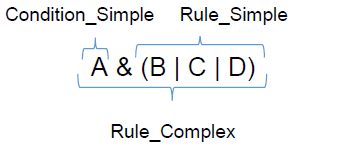
\includegraphics{images/rule}
      \caption{Example of a \code{LNM_Rule}}
  \label{fig:rule}
\end{center}
\end{figure}

IMPORTANT: The possibility to reference rules inside the rule configuration allows creating complex rules as shown in the previous image, but it requires to pay extremely attention at configuration time: recursion is possible, and it MUST BE AVOIDED.

\paragraph{Input Signals}
The Schedule Signals, input signals, are supported by LNM to create project specific conditions

Schedule signals are intended to be combined to create the project specific logic to enable the schedule state switch.


Different data types are supported for schedule signals (uint8, uint16 and boolean), and it is configurable with the parameter \code{LNM_ScheduleSignalType}.


Both SWC and Com signal sources are supported for schedule signals, and it is configurable with the parameter \code{LNM_ScheduleSignalSource}.


For each configured schedule signal, the RPort \code{RP_LNM_ScheduleSignal_<n>} is created. The user shall connect this port to the respective PPort that is providing the schedule signal.


If the configured schedule signal source is the Com, and additional port is generated,\newline \code{RP_LNM_ScheduleSignal_Av_<n>}. The user shall connect this port to the respective SUM SSM PPort that is providing the availability indication of the schedule signal.

\subsection{MSCL Configuration}
MSCL functionality can be calibrated on or off for each network through a calibration parameter \code{LNM_C_Channel_Enable_<n>}. The initial value for this calibration parameter can be set at configuration time of the LIN network \code{LNM_ChannelEnable_InitValue}. If this parameter is set to FALSE, the MSCL value will always be 0x0000.


Each bit is associated to a LIN Responder (except for the MSB that is reserved for the \code{Config bit}). Each responder bit will be set to 1 at initialization time, upon the evaluation of the corresponding \code{ResponderPresent} value.


It is possible to configure two different strategies for the evaluation of the \code{ResponderPresent} status through the configuration parameter \code{LNM_MSCL_Strategy}:
\begin{itemize}
\item \textit{Calibration}: a private calibration parameter is created for each LNM Responder. Its init value can be set at configuration time \code{LNM_C_ResponderPresent_InitValue}
\item \textit{Evaluation}: for each responder a RPort \code{RP_LNM_Cal_<XXX>_ResponderPresent} that uses a \textit{Parameter} interface is created. The user shall connect these ports to the \code{Parameter SWC} that is providing the required information, and must be sure that the data is available on the providing port before the initialization of LNM.
\end{itemize}

For each LIN network the user shall configure at least one LIN Responder, and must provide the byte and bit index in the MSCL associated to that responder (\code{LNM_MSCL_ByteIndex} and \code{LNM_MSCL_BitIndex}), accordingly to the following picture.

\begin{center}
	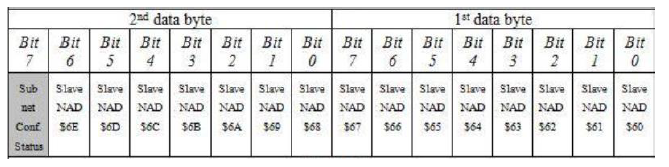
\includegraphics{images/mscl}
\end{center}

MSCL value is provided to SSM through the port \code{PP_<XXX>_LNM_SSM_MSCL}. The user shall connect this port to the respective SSM R-Port.


MSCL is stored in NvM. The user shall configure a NvM block, that has size in Byte equal to 2*n, where n is the number of configured LIN channels. Furthermore, the user shall connect the NvM service port of that block to the \code{RP_NvM_MSCL} port of LNM.

\subsection{Dcm Services}

\paragraph{DID F1BE: Commander Network Configuration List LIN}
The read operation for this DID is supported in LNM. The user shall configure this DID in its Dem configuration, enabling the services offered by LNM (\code{ConditionCheckRead} and \code{ReadData}).

The user shall connect the \code{DataService} port related to this DID to the providing \newline port \code{PP_LNM_Dcm_DID_MSCL} of LNM.

\subsection{Diagnostic}
\label{LNM Diagnostic}
In this section are described all the diagnostic functions supported by LNM. The current version of LNM implements the detection of the following DTCs:

\begin{itemize}
\item Lost Communication with LIN Responder Device
\item Loss of Communication with bus
\item Internal Electronic Failure
\item LIN Responder Device not configured
\end{itemize}


\paragraph{Lost Communication with LIN Responder Device}
The aggregation of this DTC is enabled by calibration via the \code{LNM_C_DTC_LostCommWithLinResp} parameter. For each responder the mandatory parameter \code{LNM_LossOfComm_withDevice_Timer} must be configured: this represents the debouncing timer notified to ERRH through the \code{NodeStatusIdx} interface (i.e., amount of time that ERRH must wait before requesting to Dem to set the Lost Communication with LIN Responder Device DTC).



For each configured responder the following ports are generated and must be properly connected:

\begin{itemize}
\item \code{RP_SSM_LNM_NodeTimeout_<n>}: this port shall be connected to the SSM port that provides the signal timeout notification associated to the responder
\item \code{PP_LNM_ERRH_NodeStatusIdx_<n>}: this port shall be connected to the ERRH port that is used to detect the corresponding Loss of Communication with device DTC
\end{itemize}


\paragraph{Loss of Communication with bus}
The condition to detect this DTC are always checked by LNM.
The mandatory parameter \newline \code{LNM_WupTxRetriesCommander} shall be configured (i.e., the number of retries before setting the Loss of Communication with bus DTC when the channel is not able to switch from \textit{NO\_COMMUNICATION} to \textit{FULL\_COMMUNICATION}).


For each configured LIN network the port \code{PP_LNM_ERRH_LossCommBus_<n>} is generated. This port shall be connected to the corresponding ERRH port that is checked to set the Loss of Communication with bus DTC. The mandatory parameter \code{LNM_C_DTC_LINBusOff} shall be enabled for this, otherwise any detection of Loss of Communication with Bus will be inhibited.

\paragraph{Internal Electronic Failure}
\label{sec:IEF}
The condition to detect this DTC are checked only for the configured responders that support this DTC. This DTC can be reported due to multiple consecutive reset request reported by the responder (through APINFO2 interface), or to a fault detected by the responder (through APINFO4 interface). At least one of these two mechanism shall be configured if the responder supports Internal Electronic Failure DTC.


The following parameters are used to configure Internal Electronic Failure DTC:

\begin{itemize}
\item \code{LNM_Internal_Electronic_Failure_Supported}: is a mandatory configuration parameter. Internal Electronic Failure detection will be enabled for that responder if this parameter is set to TRUE.
\item \code{LNM_IEF_APINFO2_Supported}: if this parameter is set to TRUE, the selected responder supports APINFO2 detection mechanism to set Internal Electronic Failure DTC
\item \code{LNM_IEF_APINFO4_Supported}: if this parameter is set to TRUE, the selected responder supports APINFO4 detection mechanism to set Internal Electronic Failure DTC
\item \code{LNM_IEF_Reset_Threshold}: parameter that shall be configured if APINFO2 detection mechanism is supported by the selected responder. It is the maximum number of acceptable consecutive reset request sent by the responder. When this threshold is reached, Internal Electronic Failure DTC is set
\end{itemize}


Depending on the configuration, LNM generates the following ports. Please notice that if Internal Electronic Failure is not supported by LNM, none of the following ports are generated by LNM:

\begin{itemize}
\item \code{RP_COM_LNM_APINFO2_<n>}: this port is generated only if APINFO2 detection mechanism is supported. The user shall configure a data mapping for this port to the corresponding Com signal.
\item \code{RP_COM_LNM_APINFO4_<n>}: this port is generated only if APINFO4 detection mechanism is supported. The user shall configure a data mapping for this port to the corresponding Com signal.
\item \code{PP_LNM_ERRH_IntElectFault_<n>}: this port shall be connected to the SUM\_SFFM-ERRH port that is checked to set the corresponding Internal Electronic Failure DTC.
\end{itemize}


If APINFO2 detection mechanism is supported, the runnable \code{Runnable_APINFO2_<n>}, activated by a data received event, shall be mapped to an OS task.


\paragraph{LIN Responder Device not configured}
The condition to detect this DTC are checked only for the configured responders that support this DTC.


The following parameters are used to configure LIN Responder Device not configured DTC:
\begin{itemize}
\item \code{LNM_Responder_Device_Not_Configured_Supported}: is a mandatory configuration parameter. LIN Responder Device not configured detection will be enabled for that responder if this parameter is set to TRUE.
\item \code{LNM_Config_Retries}: parameter that shall be configured if LIN Responder Device not configured is supported. This is the maximum number of acceptable consecutive configuration errors reported by the responder (through APINFO3 interface)
\end{itemize}

If the LIN Responder Device not configured DTC is supported, the following ports are generated by LNM:
\begin{itemize}
\item \code{RP_COM_LNM_APINFO3_<n>}: the user shall configure a data mapping for this port to the corresponding Com signal.
\item \code{PP_LNM_ERRH_NotConfigured_<n>}: this port shall be connected to the corresponding ERRH port that is checked to set the LIN Responder Device not configured DTC.
\end{itemize}

If LIN Responder Device not configured is supported, the runnable \code{Runnable_APINFO3_<n>}, activated by a data received event, shall be mapped to an OS task.

\subsection{Enable user functions for changing Schedule Table and Channel State}
\label{sec:UsrFuncs}

\textbf{Note:} There are two user functions which shall be implemented by user and called by SUM LNM. Each of them shall be scheduled at the same rate with Schedule or Channel rate.
\begin{itemize}
	\item \textbf{LNM\_GetRequiredSchedule}: the user function is scheduled at the rate of parameter \\LNM\_ScheduleManagement\_Period. It is used for setting the requested LIN schedule table of LIN networks.
	\item \textbf{LNM\_GetRequiredChannelState}: the user function is scheduled at the rate of parameter \\LNM\_NetworkStatus\_Period. It is used for setting the requested LIN channel state of LIN networks.
	\end{itemize}

In order to enable and use the User Functions implementation, the user shall do the following steps:

\begin{itemize}
	\item Configure the parameter \textbf{Sum\_Lnm\_ScheduleChannelUserFuncs\_Enabled} to \textbf{True}.
	\item Configure the reference to the proper LinSM Network index.
\end{itemize}

\begin{figure}[h!]
	\begin{center}
		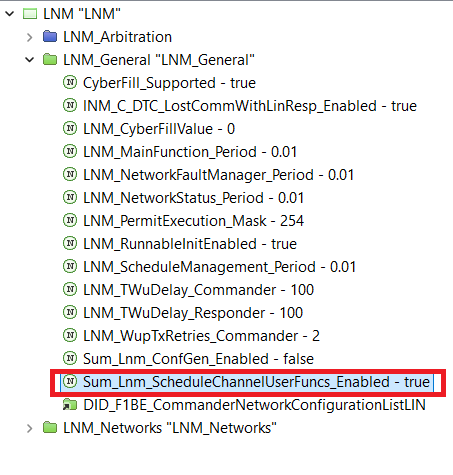
\includegraphics[width=0.6\textwidth]{images/UserFuncs}
		  \caption{RTA-SUM LNM Enable the User Functions implementation.}
	  \label{fig:cont}
	\end{center}
	\end{figure}

\begin{figure}[h!]
	\begin{center}
		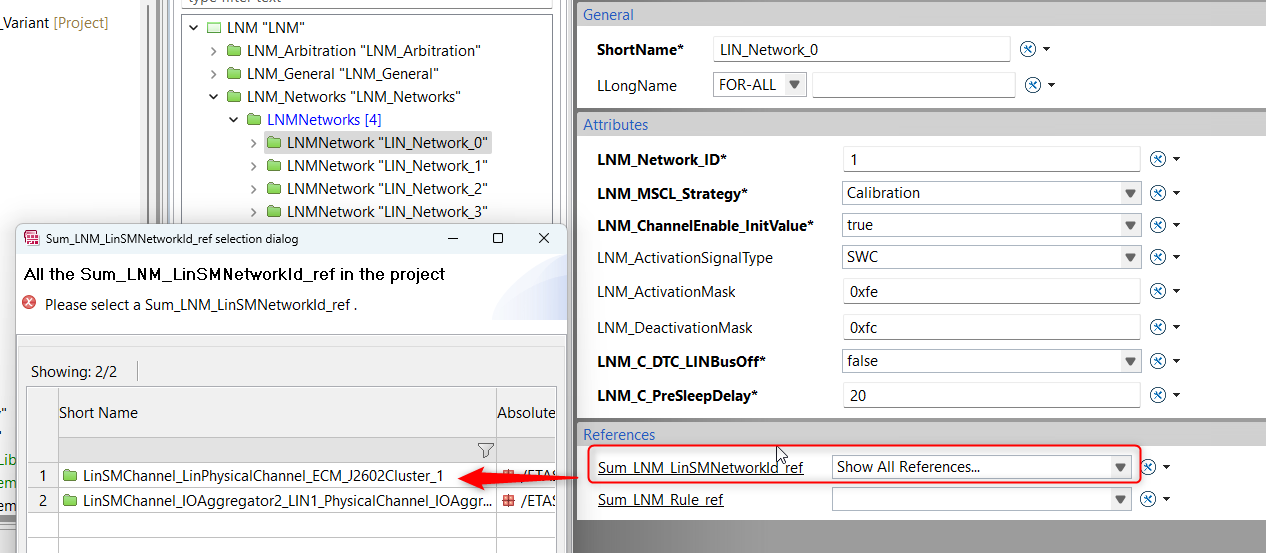
\includegraphics[width=0.6\textwidth]{images/LnmLinSMChannelRef}
		  \caption{RTA-SUM LNM channel refer to propoer LinSM Network index.}
	  \label{fig:cont}
	\end{center}
	\end{figure}
\newpage

\textbf{Note:} When the user functions are active, the user shall not need to take care of the configuration related to the LNM\_ActivationMask, LNM\_ActivationSignalType, 
LNM\_DeactivationMask and LNM\_Arbitration (Conditions, schedule signals and rules). LNM\_ScheduleManagement shall be configured to get the mode groups declaration used by BswM.

\begin{figure}[h!]
	\begin{center}
		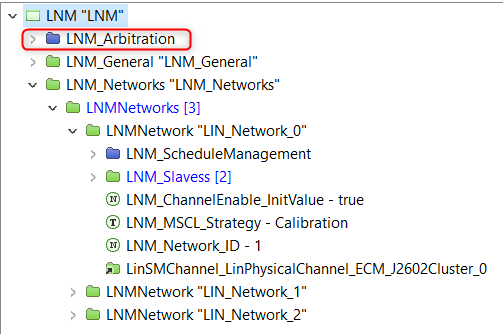
\includegraphics[width=0.6\textwidth]{images/arbitration}
		  \caption{RTA-SUM LNM Enable the User Functions implementation.}
	  \label{fig:cont}
	\end{center}
	\end{figure}
\newpage

\section{Practical configuration examples}
In this section an example of SUM LNM configuration, that can be used as reference for the user, is provided.
Example configuration requirements:
\begin{itemize}
\item Network name: LIN\_Network\_Example
\item Activation deactivation criteria: only the LSB is relevant for the activation of the LIN channel
\begin{itemize}
\item Network activation: activation signal equal to 0x01
\item Network deactivation: activation signal equal to 0x00
\end{itemize}
\end{itemize}

The following schedule table logic must be implemented

\begin{center}
	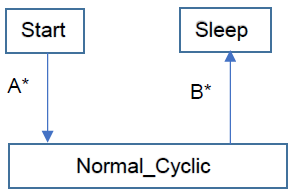
\includegraphics{images/example/f0}
\end{center}

\begin{itemize}
\item \code{ A* : (SystemPowerMode==RUN || SystemPowerMode==PROPULSION) && BrakingDetected==TRUE}
\item \code{ B* : SystemPowerMode==OFF}
\end{itemize}

\subsection{Network configuration}
\label{subsec:Network configuration}
To support the project specific activation and deactivation logic, the user has two options. For the networks whose activation criteria depends on a single activation signal, user shall configure SUM LNM in order to consider only the LSB of the activation signal as shown in Figure \ref{fig:activationSignal}. 

For the networks whose activation criteria is a rule, user shall configure SUM LNM choosing \newline\code{LNM\_ActivationSignalType} as Rule and referencing related rule in \code{Sum\_LNM\_Rule\_ref} as shown in Figure \ref{fig:activationRule}. 

\begin{figure}[h!]
	\begin{center}
		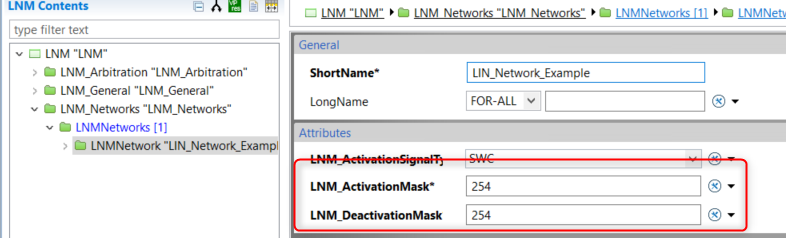
\includegraphics[width=0.8\textwidth]{images/example/f1}
		\caption{Configuration for a single activation signal}
		\label{fig:activationSignal}
	\end{center}
\end{figure}

\begin{figure}[h!]
\begin{center}
	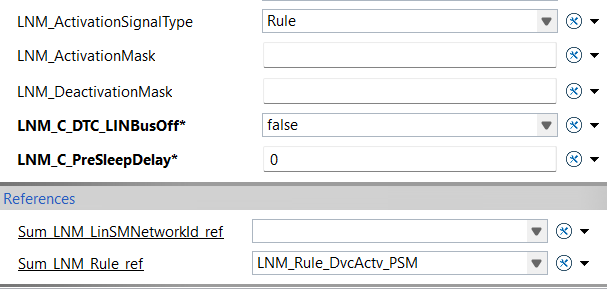
\includegraphics[width=0.8\textwidth]{images/example/f16}
		\caption{Configuration for activation rule}
	\label{fig:activationRule}
\end{center}
\end{figure}

To support the project specific schedule management, user shall configure transition rules. For the networks that are activated with a rule, user can use the activation rule also for the schedule transition, as shown in Figure \ref{fig:SchActivationRule}, in which the same activation rule is referred as in Figure \ref{fig:activationRule}. For the transition to sleep state, user shall configure a separate deactivation rule which can be equivalent to logical opposite of expression for activation rule as shown in Figure \ref{fig:SchDeactivationRule}. Details of rule configuration can be seen in the below example.

\begin{figure}[h]
	\begin{center}
		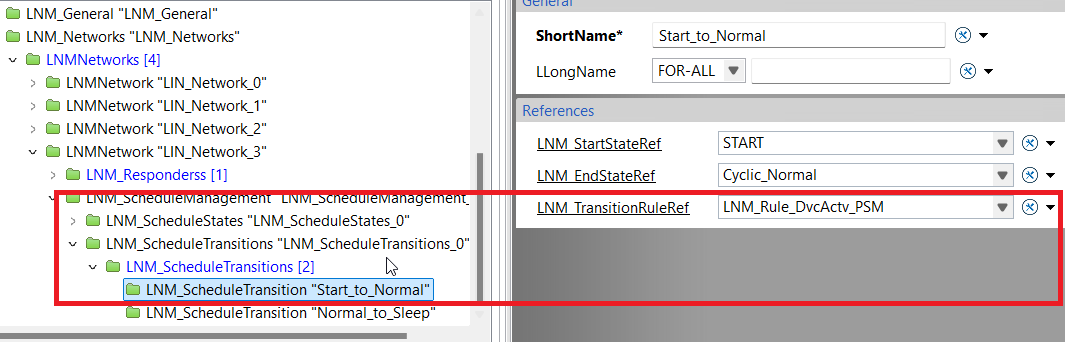
\includegraphics[width=0.8\textwidth]{images/example/f17}
		\caption{Schedule transition with activation rule}
		\label{fig:SchActivationRule}
	\end{center}
	\begin{center}
		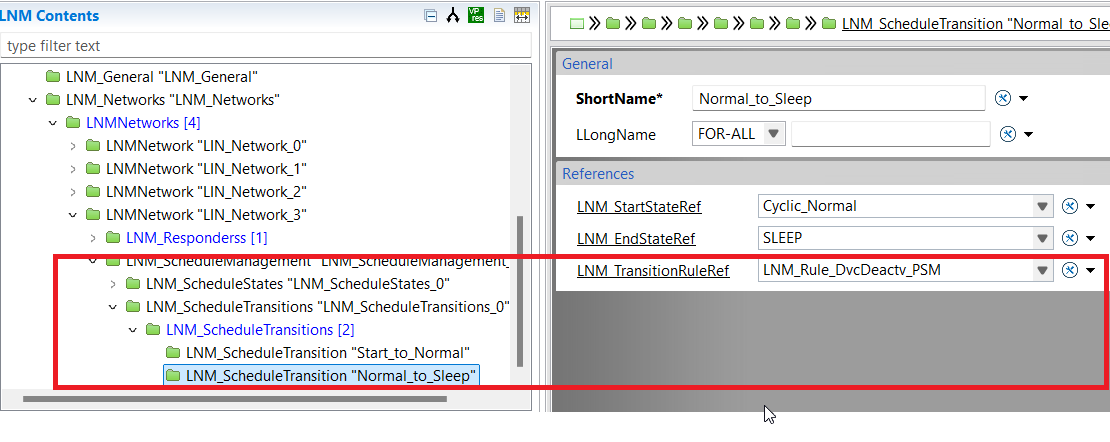
\includegraphics[width=0.8\textwidth]{images/example/f18}
		\caption{Schedule transition with deactivation rule}
		\label{fig:SchDeactivationRule}
	\end{center}
\end{figure}

For the networks whose activation criteria depends on a single activation signal, user shall configure transition rules as described below.
From the requirement it is possible to identify that two schedule signals are needed: the \textit{BrakingDetected} boolean value and the \textit{SystemPowerMode}.
The first step is to configure these schedule signals as shown in figure.
\begin{figure}[h]
	\begin{center}
		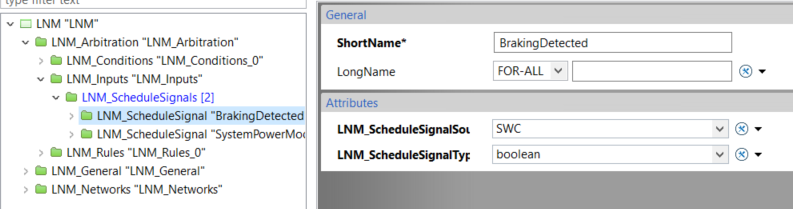
\includegraphics[width=0.8\textwidth]{images/example/f2}
	\end{center}
	\begin{center}
		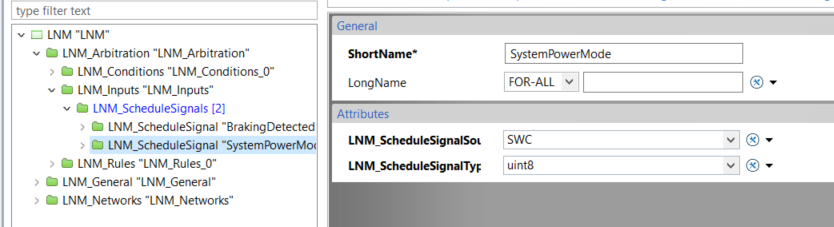
\includegraphics[width=0.8\textwidth]{images/example/f3}
	\end{center}
\end{figure}

Starting from these schedule signals, it is possible to configure all the basic conditions to be checked as shown in figure.


\begin{itemize}
\item  SystemPowerMode == RUN
\item  SystemPowerMode == PROPULSION
\item  BrakingDetected == TRUE
\item  SystemPowerMode == OFF
\end{itemize}

\begin{center}
	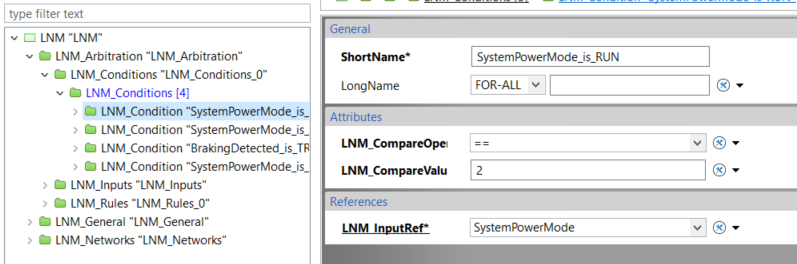
\includegraphics[width=0.8\textwidth]{images/example/f4}
\end{center}

\begin{center}
	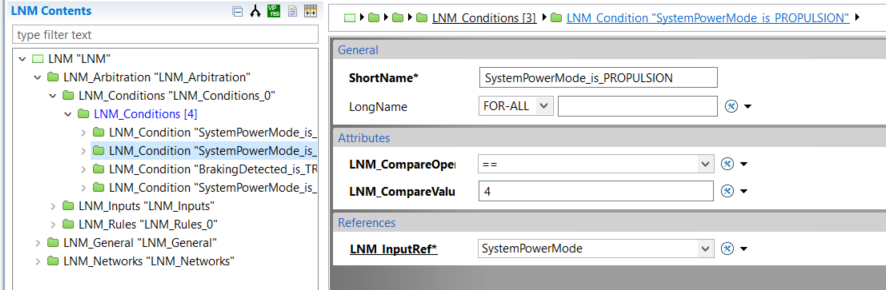
\includegraphics[width=0.8\textwidth]{images/example/f5}
\end{center}

\begin{center}
	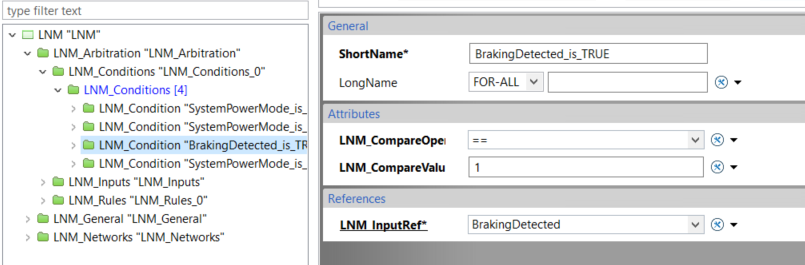
\includegraphics[width=0.8\textwidth]{images/example/f6}
\end{center}

\begin{center}
	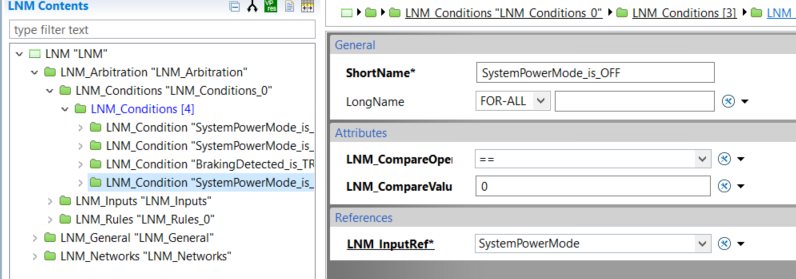
\includegraphics[width=0.8\textwidth]{images/example/f7}
\end{center}


At this point it is possible to create immediately the \code{LNM_Rule} that implements the transition B*.  Instead, an intermediate configuration is required for the rule that implements the transition A*,
since it is a complex relation of AND and OR condition.

It is possible to create a \code{LNM_Rule} that implements the condition (SystemPowerMode == RUN || SystemPowerMode == PROPULSION) as shown in figure.

\begin{center}
	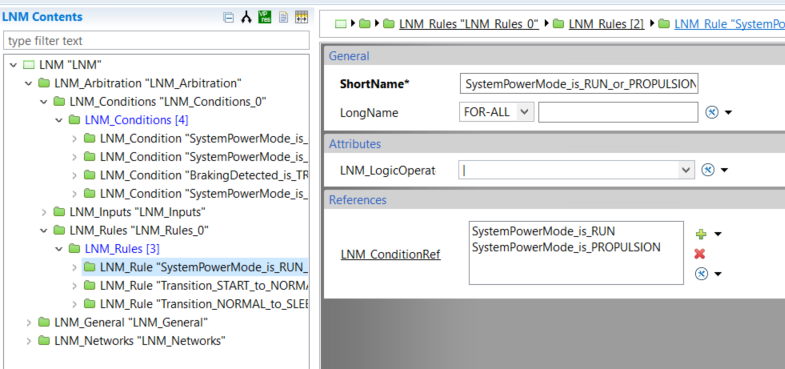
\includegraphics[width=0.8\textwidth]{images/example/f8}
\end{center}

At this point everything is in place to create a \code{LNM_Rule} that implements the logic for the transition A*.


It is now possible to configure the following rules:


\begin{itemize}
\item  \code{Transition_START_to_NORMAL} : that implements the condition A*
\item  \code{Transition_NORMAL_to_SLEEP} : that implements the condition B*
\end{itemize}


\begin{center}
	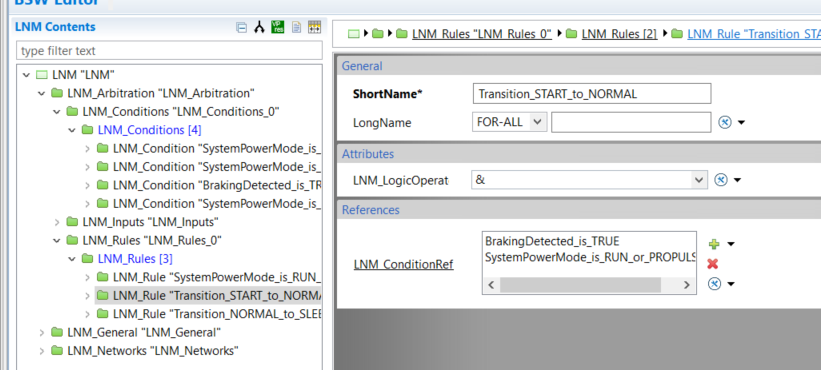
\includegraphics[width=0.8\textwidth]{images/example/f9}
\end{center}

\begin{center}
	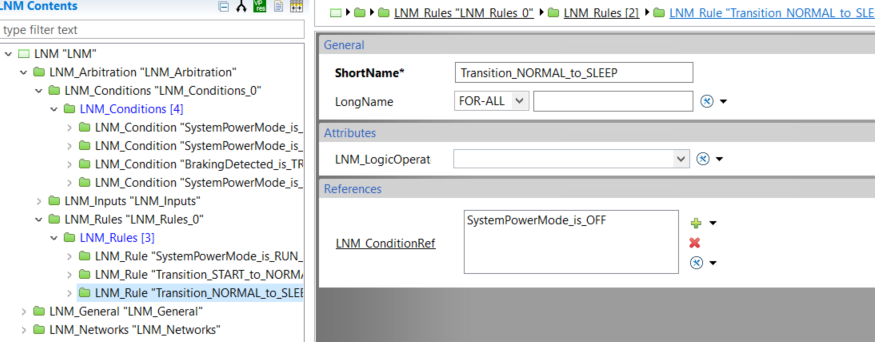
\includegraphics[width=0.8\textwidth]{images/example/f10}
\end{center}


The final step is to configure the FSM as specified in the requirements. It is needed just a single project specific state apart from the mandatory states \textit{START} and \textit{SLEEP}


\begin{center}
	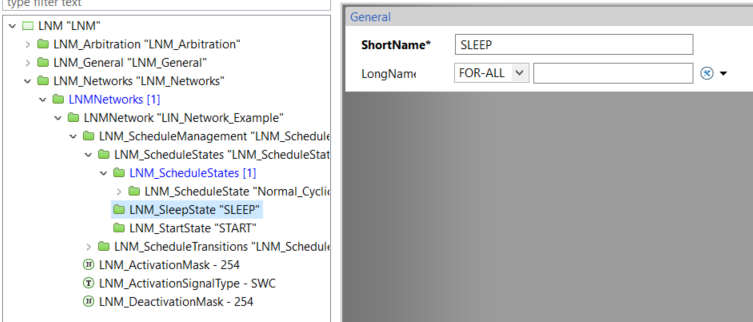
\includegraphics[width=0.8\textwidth]{images/example/f11}
\end{center}

\begin{center}
	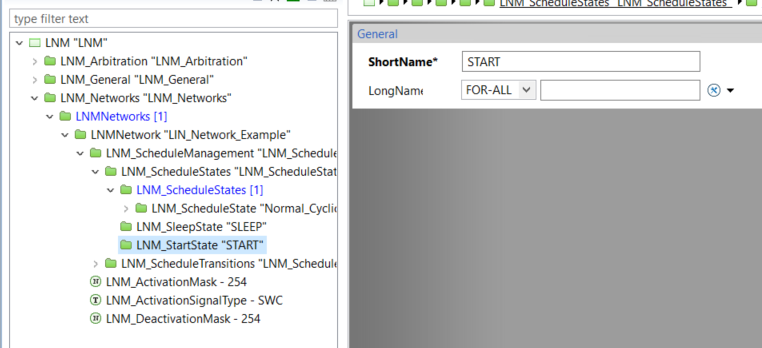
\includegraphics[width=0.8\textwidth]{images/example/f12}
\end{center}

\begin{center}
	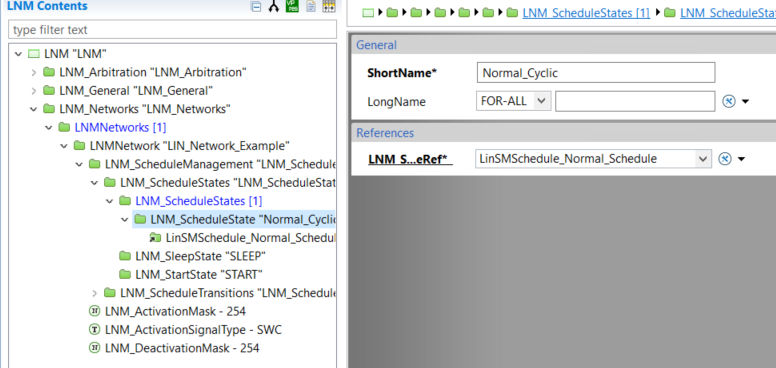
\includegraphics[width=0.8\textwidth]{images/example/f13}
\end{center}


Once that the states have been configured, it is possible to proceed with the configuration of the transitions. In this case, only two transitions are needed: A* and B*


\begin{center}
	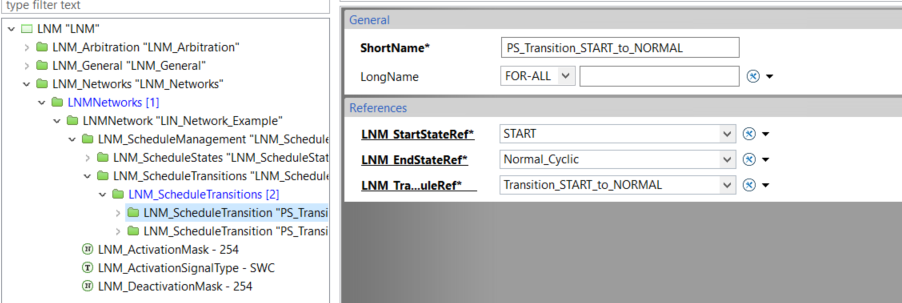
\includegraphics[width=0.8\textwidth]{images/example/f14}
\end{center}

\begin{center}
	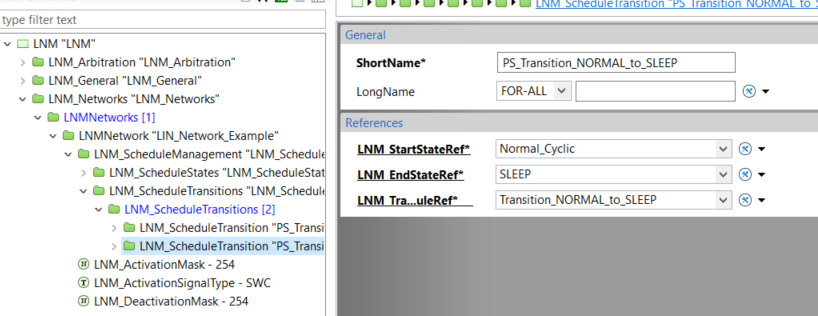
\includegraphics[width=0.8\textwidth]{images/example/f15}
\end{center}

\newpage
\subsection{ConfGen for BswM Lin Network management rules}
\label{sec:confgen}

For \textbf{Software Defined Vehicle} projects the configuration of the BswM for the ComMode and Schedule Table for a Lin Network can be automatized. 


This is possible thanks to the SUM ConfGen that starting from the System Extract it is capable of creating the \textbf{ComMode and Schedule Table EcuCValues}
for the SUM\_LNM and for the BswM.

To automate the BswM configuration the set of \textit{ModeSwitchInterface, DataTypeMappingSet and ModeDeclarationGroup} for managing ComMode and Schedule Table 
shall be created before the SUM\_LNM CodeGen, because the BswM CodeGen shall happen before the SUM\_LNM CodeGen. 

Starting from SDV the mentioned set has been moved in another file : Sum\_Lnm\_SWCD.arxml.


If the parameter \code{Sum_Lmm_ConfGen_Enabled} is set to \textbf{TRUE} the Sum\_Lnm\_SWCD.arxml is not generated by the SUM\_LNM CodeGen because is generated by the SUM ConfGen,
\textbf{so the configuration is automatized}.


If the parameter \code{Sum_Lmm_ConfGen_Enabled} is set to \textbf{FALSE} the Sum\_Lnm\_SWCD.arxml is  generated by the SUM\_LNM CodeGen and the BswM configuration shall be made by the user.


Remember to include this new file Sum\_Lnm\_SWCD.arxml in the RTE file list and that the standard SWCD has been renamed to Sum\_Lnm\_Cfg\_SWCD.arxml.



\chapter{Generic Component Interface}
\label{section:Generic Component Interface}
\begin{center}
	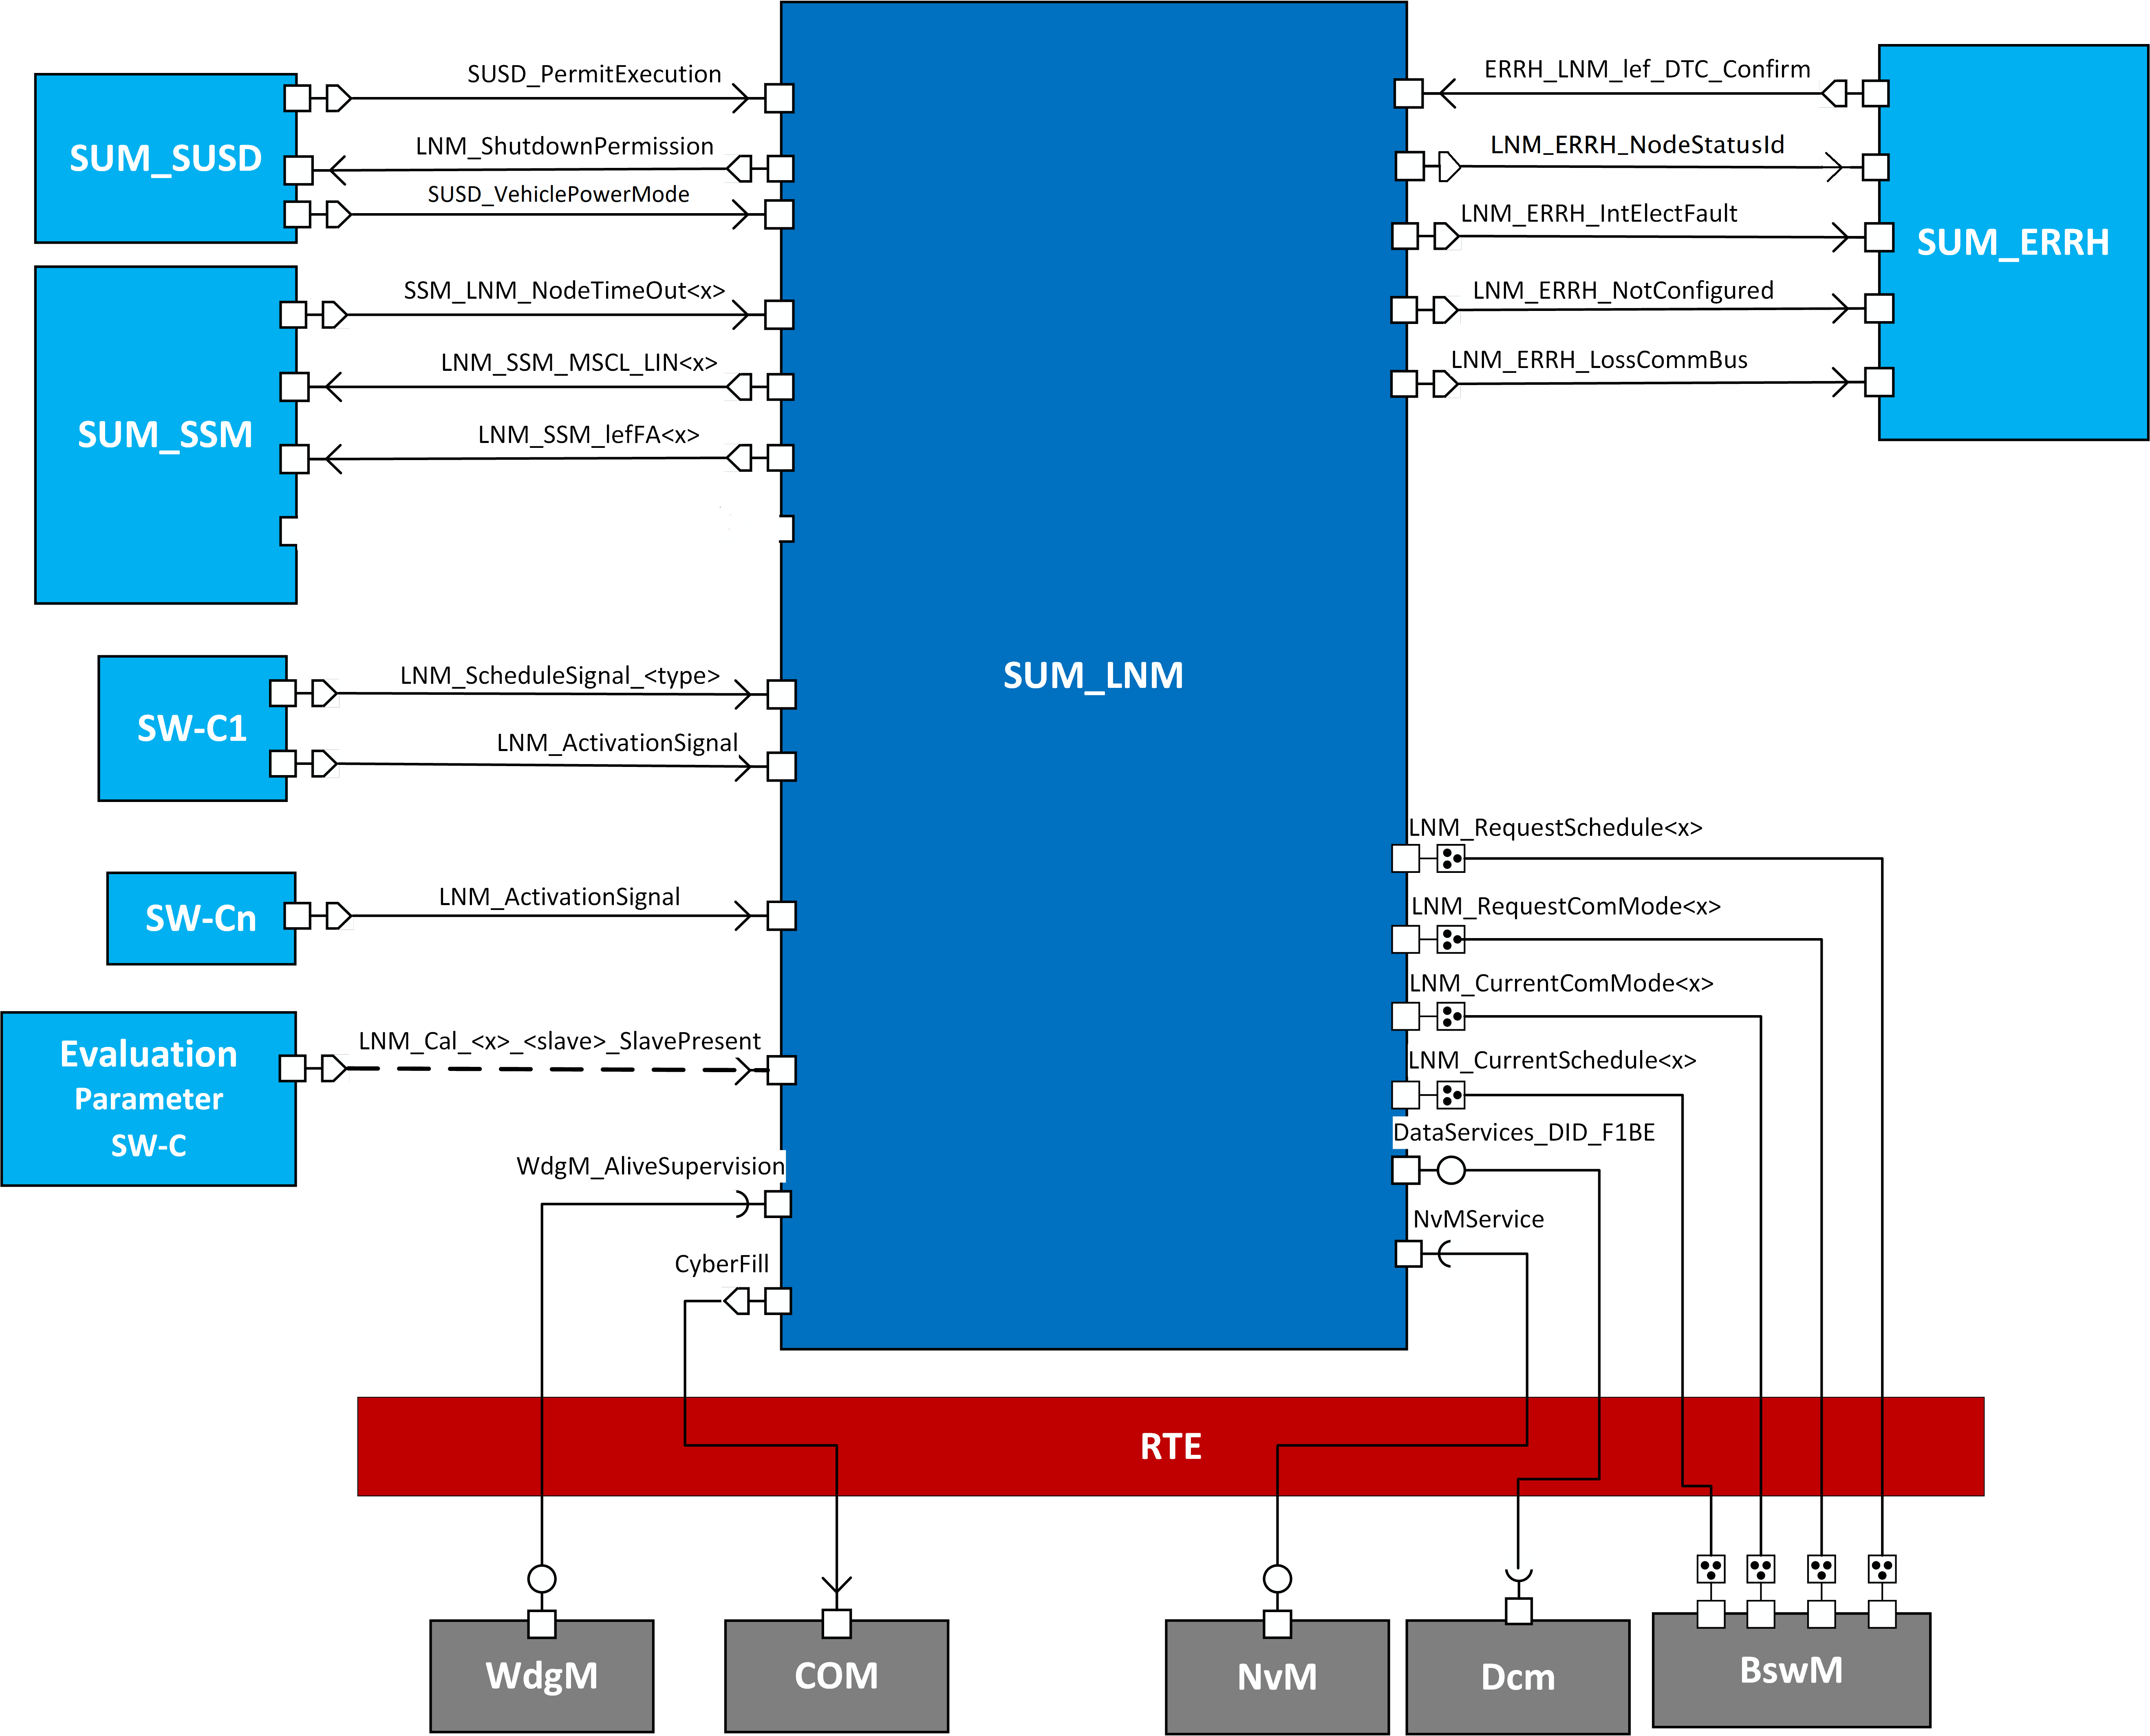
\includegraphics[width=0.9\textwidth]{images/component}
\end{center}

\input{generated/tables/port_interfaces.tex}